%\documentclass[11pt, a4paper,dalthesis]{report}    % final
%\documentclass[11pt,a4paper,dalthesis]{report}
%\documentclass[11pt,a4paper,dalthesis]{book}

\documentclass[11pt,a4paper,titlepage,oneside,openany]{article}

\pagestyle{plain}
%\renewcommand{\baselinestretch}{1.7}

\usepackage{setspace}
%\singlespacing
%\onehalfspacing
%\doublespacing
%\setstretch{1.1}

\usepackage{amsmath}
\usepackage{amssymb}
\usepackage{amsthm}
\usepackage{multicol}

\usepackage[margin=3cm]{geometry}
\usepackage{graphicx,psfrag}%\usepackage{hyperref}
\usepackage[small]{caption}
\usepackage{subfig}

\usepackage{algorithm}
\usepackage{algorithmic}
\newcommand{\theHalgorithm}{\arabic{algorithm}}

\usepackage{varioref} %NB: FIGURE LABELS MUST ALWAYS COME DIRECTLY AFTER CAPTION!!!
%\newcommand{\vref}{\ref}

\usepackage{index}
\makeindex
\newindex{sym}{adx}{and}{Symbol Index}
%\newcommand{\symindex}{\index[sym]}
%\newcommand{\symindex}[1]{\index[sym]{#1}\hfill}
\newcommand{\symindex}[1]{\index[sym]{#1}}

%\usepackage[breaklinks,dvips]{hyperref}%Always put after varioref, or you'll get nested section headings
%Make sure this is after index package too!
%\hypersetup{colorlinks=false,breaklinks=true}
%\hypersetup{colorlinks=false,breaklinks=true,pdfborder={0 0 0.15}}


%\usepackage{breakurl}

\graphicspath{{./images/}}

\usepackage[subfigure]{tocloft}%For table of contents
\setlength{\cftfignumwidth}{3em}

\input{longdiv}
\usepackage{wrapfig}


%\usepackage{index}
%\makeindex
%\usepackage{makeidx}

%\usepackage{lscape}
\usepackage{pdflscape}
\usepackage{multicol}

\usepackage[utf8]{inputenc}

%\usepackage{fullpage}

%Compulsory packages for the PhD in UL:
%\usepackage{UL Thesis}
\usepackage{natbib}

%\numberwithin{equation}{section}
\numberwithin{equation}{section}
\numberwithin{algorithm}{section}
\numberwithin{figure}{section}
\numberwithin{table}{section}
%\newcommand{\vec}[1]{\ensuremath{\math{#1}}}

%\linespread{1.6} %for double line spacing

\usepackage{afterpage}%fingers crossed

\newtheorem{thm}{Theorem}[section]
\newtheorem{defin}{Definition}[section]
\newtheorem{cor}[thm]{Corollary}
\newtheorem{lem}[thm]{Lemma}

%\newcommand{\dbar}{{\mkern+3mu\mathchar'26\mkern-12mu d}}
\newcommand{\dbar}{{\mkern+3mu\mathchar'26\mkern-12mud}}

\newcommand{\bbSigma}{{\mkern+8mu\mathsf{\Sigma}\mkern-9mu{\Sigma}}}
\newcommand{\thrfor}{{\Rightarrow}}

\newcommand{\mb}{\mathbb}
\newcommand{\bx}{\vec{x}}
\newcommand{\bxi}{\boldsymbol{\xi}}
\newcommand{\bdeta}{\boldsymbol{\eta}}
\newcommand{\bldeta}{\boldsymbol{\eta}}
\newcommand{\bgamma}{\boldsymbol{\gamma}}
\newcommand{\bTheta}{\boldsymbol{\Theta}}
\newcommand{\balpha}{\boldsymbol{\alpha}}
\newcommand{\bmu}{\boldsymbol{\mu}}
\newcommand{\bnu}{\boldsymbol{\nu}}
\newcommand{\bsigma}{\boldsymbol{\sigma}}
\newcommand{\bdiff}{\boldsymbol{\partial}}

\newcommand{\tomega}{\widetilde{\omega}}
\newcommand{\tbdeta}{\widetilde{\bdeta}}
\newcommand{\tbxi}{\widetilde{\bxi}}



\newcommand{\wv}{\vec{w}}

\newcommand{\ie}{i.e. }
\newcommand{\eg}{e.g. }
\newcommand{\etc}{etc}

\newcommand{\viceversa}{vice versa}
\newcommand{\FT}{\mathcal{F}}
\newcommand{\IFT}{\mathcal{F}^{-1}}
%\renewcommand{\vec}[1]{\boldsymbol{#1}}
\renewcommand{\vec}[1]{\mathbf{#1}}
\newcommand{\anged}[1]{\langle #1 \rangle}
\newcommand{\grv}[1]{\grave{#1}}
\newcommand{\asinh}{\sinh^{-1}}

\newcommand{\sgn}{\text{sgn}}
\newcommand{\morm}[1]{|\det #1 |}

\newcommand{\galpha}{\grv{\alpha}}
\newcommand{\gbeta}{\grv{\beta}}
%\newcommand{\rnlessO}{\mb{R}^n \setminus \vec{0}}
\usepackage{listings}
\usepackage{arydshln}

\interfootnotelinepenalty=10000

\newcommand{\sectionline}{%
  \nointerlineskip \vspace{\baselineskip}%
  \hspace{\fill}\rule{0.5\linewidth}{.7pt}\hspace{\fill}%
  \par\nointerlineskip \vspace{\baselineskip}
}

\renewcommand{\labelenumii}{\roman{enumii})}

\begin{document}

\begin{center}
  \textbf{Tutorial Sheet 6}
\end{center}

\begin{enumerate}
\item For the vectors given below, evaluate the following expressions where it is possible.
  \begin{equation*}
    \vec{u}=\left[ \begin{array}{c} 1 \\ 2 \\ 3 \end{array}\right],
    \vec{v}=\left[ \begin{array}{c} -1 \\ 0 \\ 4 \end{array}\right],
    \vec{x}=\left[ \begin{array}{c} 3 \\ 4 \end{array}\right],
    \vec{y}=\left[ \begin{array}{c} -4 \\ 3 \end{array}\right],
    \vec{w}=\left[ \begin{array}{c} 1 \\ 0\\ 2 \\ -5 \end{array}\right],
    \vec{z}=\left[ \begin{array}{c} 2 \\ 2 \\ 2 \\ 3 \end{array}\right]
        \end{equation*}
        \begin{multicols}{3}
          \begin{enumerate}
          \item $2\vec{u} + 3\vec{v}$
          \item $3\vec{u} - \vec{v}$
          \item $\vec{x} + 3\vec{v}$
          \item $2\vec{z} - \vec{w}$
          \item $\vec{u}+\vec{x}$
          \item $\vec{v}+\vec{w}$
          \item $\vec{u}\cdot \vec{v}$
          \item $\left(2\vec{u}\right)\cdot \left(3\vec{v}\right)$
          \item $\vec{x}\cdot \vec{y}$
          \item $\vec{w} \cdot \vec{z}$
          \item $\vec{w} \cdot (\vec{z}+\vec{w})$
          \item $|\vec{x}|$
          \item $|\vec{w}|$
          \item $|\vec{y}|+|\vec{w}|$
          \end{enumerate}
        \end{multicols}

\item
  Calculate the angles between the pairs $\vec{u},\vec{v}$, $\vec{x},\vec{y}$, and $\vec{w},\vec{z}$ from the previous question. Give your answers in both radians and degrees.

\item
  For the matrices below, evaluate the following expressions where it is possible.
  \begin{equation*}
    A=\left[ \begin{array}{cc} 1  & 2 \\ 3 & 4 \end{array}\right],
    B=\left[ \begin{array}{cc} -2  & 0 \\ 1 & -7 \end{array}\right],
    C=\left[ \begin{array}{ccc} 3  & 2 & -2 \\ 4 & 8 & 2 \end{array}\right],
    D=\left[ \begin{array}{ccc} 3  & 2 & -2 \\ 4 & 8 & 2 \end{array}\right],
  \end{equation*}
  \begin{equation*}
    E=\left[ \begin{array}{ccc} 1  & 2 & 3 \\ 4 & 5 & 6 \\ 7 & 8 & 9 \end{array}\right],
    F=\left[ \begin{array}{ccc} -1  & 0 & 2 \\ 3 & 4 & 1 \\  3 & 1 & 0 \end{array}\right],
  \end{equation*}
  %-------------------%
    \begin{equation*}
G=\left[ \begin{array}{cc}3 & 4 \\1 & 2 \\2 &-1 \\ \end{array}\right],
H=\left[ \begin{array}{ccc}3 & 4 & 3\\1 & 2 & 2\\ \end{array}\right],
I=\left[ \begin{array}{ccc}2 & 2 & 1\\ \end{array}\right],
  \end{equation*}
  %-------------------%
    \begin{equation*}
J=\left[ \begin{array}{c}
3\\
1\\
1\\ \end{array}\right],
K=\left[ \begin{array}{ccc}
2 & 1 & 3\\1 & 2 & 2\\2 & 1 & 0\\\end{array}\right], 
  \end{equation*}
  %-------------------------------%
  \begin{multicols}{3}
    \begin{enumerate}
    \item $2A+3B$
    \item $3C-D$
    \item $8A+4C$
    \item $2000A+3000B$
    \item $E-F$
    \item $A\vec{x}$
    \item $B\vec{x}$
    \item $A\vec{y}+B\vec{x}$
    \item $A\vec{u}$
    \item $C\vec{x}$
    \item $C\vec{w}$
    \item $E\vec{u}$
    \item $E\vec{w}-\vec{F}\vec{w}$

    \end{enumerate}
  \end{multicols}

\end{enumerate}
\end{document}
\pagebreak

\begin{center}
  \textbf{Tutorial Sheet 7}
\end{center}

\begin{enumerate}
\item
  For each of the following systems of linear equations, write down the corresponding coefficient matrix $A$, vector of unknowns $\vec{x}$, and vector of right hand sides $\vec{b}$ so that the system can be expressed in the form $A\vec{x}=\vec{b}$
  \begin{multicols}{3}
    \begin{enumerate}
      \item
        \begin{align*}
          2x+3y&=1\\
          5x+7y&=3
        \end{align*}
      \item\begin{align*}
          2x+3y+4z&=1\\
          x-2y+2z&=7\\
          3x+2y+z&=0.2
        \end{align*}
        \item
        \begin{align*}
          3x+y+z&=1\\
          y+4z&=-4\\
          x-y&=2
        \end{align*}
    \end{enumerate}
  \end{multicols}
\item
\end{enumerate}
%\begin{wrapfigure}{r}{0.5\textwidth}
%    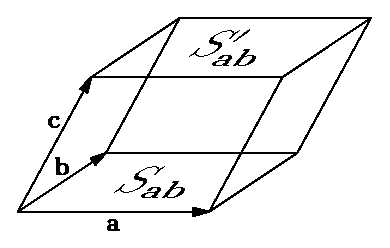
\includegraphics[width=0.5\textwidth]{par3_tut}
%    \vspace{-5em}
%\end{wrapfigure}

Let the vectors $\vec{a},\vec{b},\vec{c}$ be given by
  \begin{equation*}
    \vec{a}=\left[ \begin{array}{c} 2 \\ 0 \\ 0 \end{array}\right],
    \vec{b}=\left[ \begin{array}{c} 2 \\ 1 \\ 0 \end{array}\right],
    \vec{c}=\left[ \begin{array}{c} 2 \\ 0 \\ 1 \end{array}\right]
  \end{equation*}
  These vectors span a three dimensional parallelopiped as shown in the figure to the right.

  \begin{enumerate}
    \renewcommand{\theenumi}{\roman{enumi})}
    \renewcommand{\labelenumi}{\theenumi}
  {\setlength\itemindent{3em} \item
    Find the area of the parallelogram $S_{\vec{a}\vec{b}}$ which is spanned by the vectors $\vec{a}$ and $\vec{b}$. Hence state the area of the parallelogram $S_{\vec{a}\vec{b}}'$ on the opposite side of the parrallelopiped.}
  {\setlength\itemindent{3em} \item
    Find the areas of the parallelograms $S_{\vec{b}\vec{c}}$ and $S_{\vec{a}\vec{c}}$ spanned by the relevant pairs of vectors and hence find the total surface area of the parrallelopiped.}
  {\setlength\itemindent{3em} \item
    Find the signed volume of the parrallelopiped.}
  \end{enumerate}

\begin{enumerate}
\setcounter{enumi}{2}
\item
  Rotate the point $\vec{x}=\left[ \begin{array}{c} 1 \\ 3 \end{array}\right]$ anti-clockwise $\frac{\pi}{4}$ radians about the point $\vec{p}=\left[ \begin{array}{c} 2 \\ 2 \end{array}\right]$.
\item
  Rotate the line segment with endpoints $\vec{x}=\left[ \begin{array}{c} 1 \\ 3 \end{array}\right]$ and $\vec{y}=\left[ \begin{array}{c} 3 \\ 3 \end{array}\right]$ anti-clockwise $\frac{\pi}{2}$ radians about the point $\vec{p}=\left[ \begin{array}{c} 2 \\ 2 \end{array}\right]$. Give the new endpoints $\vec{x}'$ and $\vec{y}'$ of the rotated line segment.
\end{enumerate}

\end{document}

%%% Local Variables:
%%% mode: latex
%%% TeX-master: t
%%% End:
